
\section{\hard\ \trSeparated{}性与\trProperness{}的\trValuativeCriteria}

（本节之所以被放在这里，唯一的理由是我们需要离散\trValuationRing{}的理论。）

在合理的情形下，只须检验从\trValuationRing{}的谱出发的映射，便足以验证分离性。这一做法有四点招人喜欢之处（哪怕你从不使用它）。第一，它对分离态射的长相给出了有用的直觉。第二，既然我们通过映入概形的映射来理解概形（\trYoneda{}哲学），我们自然也会期待通过把概形之间的某些映射映入其中来理解态射——而出现在\trValuativeCriteria{}中的那幅图，正可以由此得到解读。第三条具体的理由是：命题所述的两个方向中，有一个要容易得多（它是「既约到分离」定理~11.3.2 的特例；见\mbox{练习~13.7.A}），而这正是我们将会反复使用的那个方向。最后，这条判别法非常有用！

类似地，\trProperness{}也有一条\trValuativeCriteria。

在本节中，我们将与这些\trValuativeCriteria{}见面；但除了勾画其中一个结果（\trSeparated{}性的\trValuativeCriteria{}的\trDVR{}版本）的证明之外，我们不会给出证明，而以满足于给出参考文献了事。这个有争议的决定有两个理由。第一，这些证明需要发展一些涉及\trValuationRing{}的交换代数，而我们除此之外并不需要它们。第二，在本书后文中，我们不会以任何实质性的、非用不可的方式使用这些结果。

我们从一个\trSeparated{}性的\trValuativeCriteria{}入手，它适用的情形足以满足大多数人的兴趣：诺特概形之间的有限型\trMorphism。随后，我们会为更一般的读者给出一个更一般的版本。

\textbf{13.7.1.\ \trhTheorem{}（\trSeparated{}性的\trValuativeCriteria，\trDVR{}版本；见\cref{fig:valuative-criterion-separatedness}）。}\ ——\ \emph{设 $\pi\colon X\to Y$ 是局部诺特概形之间的一个有限型\trMorphism。则 $\pi$ 是\trSeparated{}的，当且仅当下述条件成立：对任何\trDVR{} $A$，以及任何形如}
\begin{equation*}\tag{13.7.1.1}\label{eq:valuative-criterion-diagram}
\begin{tikzcd}[row sep=3.2em]
\Spec K(A) \ar[rr] \ar[d, hook, "\text{开浸入}"'] & & X \ar[d, "\pi"] \\
\Spec A \ar[rr] & & Y
\end{tikzcd}
\end{equation*}
\emph{的图（其中左边的竖直\trMorphism{}对应于包含映射 $A\hookrightarrow K(A)$），使得图}
\begin{equation*}\tag{13.7.1.2}\label{eq:valuative-criterion-lift}
\begin{tikzcd}[row sep=3.2em]
\Spec K(A) \ar[rr] \ar[d, hook, "\text{开浸入}"'] & & X \ar[d, "\pi"] \\
\Spec A \ar[rr] \ar[urr, dotted, "\leq 1"] & & Y
\end{tikzcd}
\end{equation*}
\emph{交换的\trMorphism{} $\Spec A\to X$ 至多只有一个。}

证明背后的想法在 \S13.7.3 中解释。其中一个方向我们马上就能证明，就在下一道练习里。

\textbf{13.7.A.（练习：容易的方向）}\quad 请用「既约到分离」定理~11.3.2 证明定理中的一个方向：若 $\pi$ \trSeparated，则这条\trValuativeCriteria{}成立。

\begin{figure}[htbp]
\centering
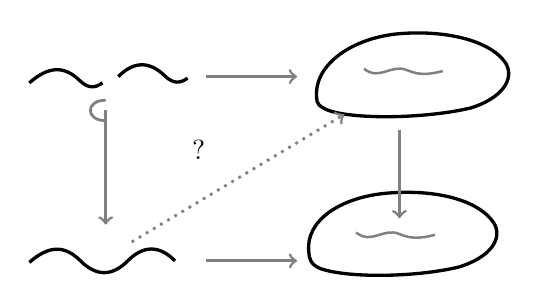
\begin{tikzpicture}[line width=1.2pt]
  \draw (-2.55,1.30) .. controls (-2.30,1.52) and (-2.10,1.52) .. (-1.90,1.32) .. controls (-1.80,1.23) and (-1.72,1.23) .. (-1.62,1.30);
  \draw (-1.42,1.38) .. controls (-1.22,1.58) and (-1.02,1.58) .. (-0.82,1.38) .. controls (-0.72,1.29) and (-0.64,1.29) .. (-0.54,1.36);
  \draw (-2.55,-0.98) .. controls (-2.30,-0.76) and (-2.10,-0.76) .. (-1.90,-0.96) .. controls (-1.70,-1.16) and (-1.50,-1.16) .. (-1.30,-0.96) .. controls (-1.10,-0.76) and (-0.90,-0.76) .. (-0.70,-0.96);
  \draw (1.10,1.10) .. controls (1.05,1.50) and (1.50,1.85) .. (2.10,1.92) .. controls (2.70,1.98) and (3.30,1.85) .. (3.50,1.55) .. controls (3.62,1.35) and (3.45,1.10) .. (3.05,0.98) .. controls (2.50,0.85) and (1.60,0.83) .. (1.25,0.95) .. controls (1.12,1.00) and (1.10,1.05) .. (1.10,1.10);
  \draw[gray,line width=0.9pt] (1.70,1.48) .. controls (1.90,1.32) and (2.05,1.55) .. (2.25,1.46) .. controls (2.40,1.40) and (2.50,1.40) .. (2.70,1.45);
  \draw (1.00,-0.85) .. controls (0.95,-0.45) and (1.40,-0.15) .. (2.00,-0.10) .. controls (2.60,-0.05) and (3.15,-0.18) .. (3.35,-0.48) .. controls (3.47,-0.68) and (3.30,-0.92) .. (2.90,-1.04) .. controls (2.35,-1.17) and (1.50,-1.18) .. (1.15,-1.06) .. controls (1.02,-1.01) and (1.00,-0.92) .. (1.00,-0.85);
  \draw[gray,line width=0.9pt] (1.60,-0.60) .. controls (1.80,-0.76) and (1.95,-0.53) .. (2.15,-0.62) .. controls (2.30,-0.68) and (2.40,-0.68) .. (2.60,-0.63);
  \draw[gray,line width=1pt,->] (-0.30,1.38) -- (0.85,1.38);
  \draw[gray,line width=1pt,->] (-0.30,-0.96) -- (0.85,-0.96);
  \draw[gray,line width=1pt,->] (-1.58,0.95) -- (-1.58,-0.50);
  \draw[gray,line width=1pt] (-1.58,1.08) .. controls (-1.84,1.08) and (-1.84,0.82) .. (-1.58,0.82);
  \draw[gray,line width=1pt,->] (2.15,0.70) -- (2.15,-0.42);
  \draw[gray,line width=1pt,->,dotted] (-1.25,-0.72) -- (1.45,0.90);
  \node at (-0.40,0.45) {$?$};
\end{tikzpicture}
\caption{\trSeparated{}性的\trValuativeCriteria。（依原书手绘图重绘。）}\label{fig:valuative-criterion-separatedness}
\end{figure}

\textbf{13.7.B.（练习）}\quad 设 $X$ 是一条整的诺特分离\trCurve。若 $p\in X$ 是一个正则的\trClosedPoint，则 $\OO_{X,p}$ 是一个\trDVR，于是每个正则点都在 $K(X)$ 上给出一个离散\trValuation。请用上一道练习证明：不同的点给出不同的离散赋值。

下面是这条\trValuativeCriteria{}背后的直觉（见\cref{fig:valuative-criterion-separatedness}）。我们把一个\trDVR{} $A$ 的 $\Spec$ 想成「一条\trCurve{}的\trGerm」，把 $\Spec K(A)$ 想成「挖去原点的\trGerm」（尽管它只是一个点！）。于是，这条\trValuativeCriteria{}说的是：若我们有一个从\trCurve{}的\trGerm{}到 $Y$ 的映射，并且有这个映射在挖去原点之处到 $X$ 的一个提升，那么把它从整个\trGerm{}提升起来的方式至多只有一种。当 $Y$ 是一个域的谱时，你可以把这理解为：单参数族的极限（若存在）必唯一。

例如，这抓住了 $k$ 上原点加倍了的\trAffineLine{}的映射毛病何在（\cref{fig:line-doubled-origin}）：我们取 $\Spec A$ 为\trAffineLine{}在原点处的\trGerm，考虑挖去原点的\trGerm{}到原点加倍了的\trAffineLine{}的映射。于是，这个映射延拓过原点的方式有两种选择。

\begin{figure}[htbp]
\centering
\begin{tikzpicture}[line width=1.2pt]
  \draw (-3.35,1.55) -- (-2.40,1.55);
  \draw (-2.15,1.55) -- (-1.20,1.55);
  \draw (0.60,1.55) -- (3.35,1.55);
  \draw[line width=1.1pt,fill=white] (2.10,1.55) circle (0.085);
  \draw (-3.35,-1.50) -- (-1.20,-1.50);
  \fill (2.10,-1.50) circle (0.075);
  \draw[gray,line width=1pt,->] (-0.60,1.55) -- (0.32,1.55);
  \draw[gray,line width=1pt,->] (-0.60,-1.50) -- (0.32,-1.50);
  \draw[gray,line width=1pt,->] (-2.15,1.30) -- (-2.15,-1.25);
  \draw[gray,line width=1pt,->] (2.10,1.30) -- (2.10,-1.25);
  \draw[gray,line width=1pt,->] (-1.88,-1.02) .. controls (-0.60,-0.15) and (0.50,0.70) .. (1.52,1.30);
  \draw[gray,line width=1pt,->] (-1.62,-1.26) .. controls (0.05,-0.60) and (1.10,0.15) .. (1.82,1.02);
  \node at (-1.15,0.38) {$\pi$};
  \node at (0.78,-0.55) {$\pi'$};
  \node at (0.02,0.10) {两种选择};
\end{tikzpicture}
\caption{原点加倍了的\trAffineLine{}不满足\trSeparated{}性的\trValuativeCriteria。（你也许会注意到\cref{fig:nonseparated-agreement}就嵌在这幅图里。）（依原书手绘图重绘。）}\label{fig:line-doubled-origin}
\end{figure}

\textbf{13.7.C.（练习）}\quad 请把这件事说精确：证明 $k$ 上原点加倍了的\trAffineLine{}到 $\Spec k$ 的映射不满足\trSeparated{}性的\trValuativeCriteria。（更早的论证见于\mbox{练习~11.2.I} 与\mbox{练习~11.3.C}。）

\textbf{13.7.2.}\ \extrahard\ \emph{行家注记：\trModuliSpace{}与\trSeparated{}性的\trValuativeCriteria。}\quad 若 $Y=\Spec k$，而 $X$ 是某类对象的（精细的）\trModuliSpace（这个术语我们在此不定义），那么 $X$（在 $\Spec k$ 上）的\trSeparatedness{}问题便有一个自然的解读：给定一个由「被刺穿的\trDVR」参数化的、由你的那些对象组成的\trFamily，把它延拓过闭点的方式是否总至多只有一种？

\textbf{13.7.3.}\ \emph{定理~13.7.1（\trSeparated{}性的\trValuativeCriteria{}的\trDVR{}版本）在簇情形下证明背后的想法。}\quad （一个方向已在\mbox{练习~13.7.A}中完成。）若 $\pi$ 不\trSeparated，我们的目标便是造出一幅形如 \eqref{eq:valuative-criterion-diagram}、且能以不止一种方式补全成 \eqref{eq:valuative-criterion-lift} 的图。若 $\pi$ 不\trSeparated，则 $\delta\colon X\to X\times_Y X$ 是一个并非闭嵌入的\trLocallyClosedEmbedding。

\textbf{13.7.D.（练习）}\quad 证明：你可以找到不在 $X\times_Y X$ 的对角线 $\Delta$ 中的点 $p$，以及 $\Delta$ 中的点 $q$，使得 $p\in\overline{q}$，而且不存在「介于 $p$ 与 $q$ 之间」的点（不存在异于 $p$ 与 $q$ 且满足 $p\in\overline{r}$ 与 $r\in\overline{q}$ 的点 $r$）。（\cref{ex:constructible-stable-specialization} 或许会带来一些启发。）

令 $Q$ 为给 $\overline{q}$ 赋以诱导的既约子概形结构所得的概形。令 $B=\OO_{Q,p}$ 为 $Q$ 在 $p$ 处的\trLocalRing。

\textbf{13.7.E.（练习）}\quad 证明：$B$ 是一个维数为 $1$ 的诺特局部整环。

若 $B$ 正则，那么我们就大功告成了：把包含态射 $Q\to X\times_Y X$ 与两个投射复合，诱导出同一个态射 $q\to X$（即 $\Spec\kappa(q)\to X$），但到 $B$ 上的延拓却彼此不同，其原因恰恰在于 $p$ 不在对角线之中。为了完成证明，需要证明 $B$ 的\trNormalization{}是诺特的；这正是我们需要「我们处理的是簇」这一假设之处，以便援引\mbox{练习~10.7.M}。然后在 $p$ 上方的任何一个素处取局部化（由 Lying Over 定理~8.2.5，这样的素是存在的），便得到所要的\trDVR{} $A$。

至于真正货真价实的证明，见 [Stacks, tag~0207] 或 [Gr-EGA, II.7.2.3]。

用更加强力的方式调用交换代数，我们便能在限制性假设弱得多的情形下证明一条\trValuativeCriteria。

\textbf{13.7.4.\ \trhTheorem{}（\trSeparated{}性的\trValuativeCriteria）。}\ ——\ \emph{设 $\pi\colon X\to Y$ 是一个拟分离\trMorphism。则 $\pi$ 是\trSeparated{}的，当且仅当：对任何\trValuationRing{} $A$，以及任何形如 \eqref{eq:valuative-criterion-diagram} 的图，使得 \eqref{eq:valuative-criterion-lift} 交换的\trMorphism{} $\Spec A\to X$ 至多只有一个。}

既然我已经没能把\trDVR{}版本证明完整，我也就提不起兴致去证明这个更难的事实了。其中一个方向——$\pi$ \trSeparated{}蕴涵判别法成立——其证明与\mbox{练习~13.7.A}中的论证完全一样。完整的证明见 [Stacks, tags~01KY 与 01KZ] 或 [Gr-EGA, II.7.2.3]。

\textbf{13.7.5.\ （泛闭性与）\trProperness{}的\trValuativeCriteria。}\quad \trProperness{}也有一条\trValuativeCriteria。它在哲学上有用，有时也直接有用，尽管我们并不需要它。它自然地来自\trSeparated{}性的\trValuativeCriteria{}与泛闭性的\trValuativeCriteria{}二者的结合。

\textbf{13.7.6.\ \trhTheorem{}（泛闭性与\trProperness{}的\trValuativeCriteria，\trDVR{}版本）。}\ ——\ \emph{设 $\pi\colon X\to Y$ 是局部诺特概形之间的一个有限型\trMorphism。则 $\pi$ 是\trUniversallyClosed{}的（相应地，固有的），当且仅当：对任何\trDVR{} $A$，以及任何图 \eqref{eq:valuative-criterion-diagram}，使得 \eqref{eq:valuative-criterion-lift} 交换的\trMorphism{} $\Spec A\to X$ 至少有一个（相应地，恰有一个）。}

证明见 [Gr-EGA, II.7.3.8]、[Ha1, Thm.~II.4.7] 或 [Gr-EGA$'$, I.5.5]。与定理~13.7.1 作一番比较，你就会相信这三条判别法自然地构成一个家族。

当 $Y$ 是一个域时，你可以把\trProperness{}的\trValuativeCriteria{}理解为：固有簇中单参数族的极限总是存在，而且唯一。这是对\trProperness{}这一观念的一个有用的直觉。

\textbf{13.7.F.（容易的练习）}\quad 请用\trProperness{}的\trValuativeCriteria{}证明：若 $A$ 是诺特环，则 $\mathbb{P}^n_A\to\Spec A$ 是固有的。（别被愚弄了：正因为这要用到\trValuativeCriteria，这是证明我们在定理~11.4.5 中已经证明过的事实的一条困难途径。）

\textbf{13.7.G.（练习；与\mbox{练习~13.7.B} 相对照）}\quad 设 $X$ 是一条不可约正则（诺特）\trCurve，在域 $k$ 上（相应地，在 $\mathbb{Z}$ 上）固有。请描述 $K(X)$ 上那些使 $k$（相应地，$\mathbb{Z}$）的元素赋值为 $0$ 的离散赋值与 $X$ 的闭点之间的一个双射。

\textbf{13.7.7.}\ \emph{行家注记。}\quad 有一个与\trSeparated{}性情形（注记~13.7.2）类似的模理论式解读：$X$ 是固有的，当且仅当把一个定义在\trDVR{}的刺穿谱上的\trFamily{}填补完整的方式总恰有一种。

\textbf{13.7.8.}\quad 最后，给出泛闭性与\trProperness{}的\trValuativeCriteria{}的一个更花哨的版本。

\textbf{13.7.9.\ \trhTheorem{}（泛闭性与\trProperness{}的\trValuativeCriteria）。}\ ——\ \emph{设 $\pi\colon X\to Y$ 是拟分离、有限型（因而拟紧）的\trMorphism。则 $\pi$ 是\trUniversallyClosed{}的（相应地，固有的），当且仅当下述条件成立。对任何\trValuationRing{} $A$ 与任何形如 \eqref{eq:valuative-criterion-diagram} 的图，使得 \eqref{eq:valuative-criterion-lift} 交换的\trMorphism{} $\Spec A\to X$ 至少有一个（相应地，恰有一个）。}

显然，\trProperness{}的\trValuativeCriteria{}是\trSeparated{}性的\trValuativeCriteria{}（定理~13.7.4）与泛闭性的\trValuativeCriteria{}二者的推论。证明见 [Stacks, tag~01KF] 或 [Gr-EGA, II.7.3.8]。

\textbf{13.7.10.\ 一般\trValuationRing{}的重要性。}\quad 尽管我们只深入讨论过\trDVR，但一般的\trValuationRing{}不应被视作事后补想的东西。\trSerre{}在一封信中向\trGrothendieck{}申明了这番道理\footnote{译注：来信按原书照录法语原文；紧随其后的一段中文，是笔者对作者英译的转译，个别字句从法文原信。}，[GrS, p.~125]：
\begin{quote}\itshape
Tu es bien sévère pour les Valuations!
Je persiste pourtant à les garder, pour plusieurs raisons:
d'abord une pratique: n rédacteurs ont sué dessus,
il n'y a rien à reprocher au fourbi,
on ne doit pas le vider
sans raisons très sérieuses (et tu n'en as pas).\,\ldots\
Même un noethérien impénitent a besoin
des valuations discrètes, et de leurs extensions;
en fait, Tate, Dwork, et tous les gens p-adiques
te diront qu'on ne peut se limiter au cas discret
et que le cas de rang 1 est indispensable;
à ce moment, les méthodes noethériennes
deviennent un vrai carcan,
et on comprend beaucoup mieux
en rédigeant le cas général
que uniquement le cas de rang 1.\,\ldots\
Il n'y a pas lieu d'en faire un plat,
bien sûr,
et c'est pourquoi j'avais vivement
combattu le plan Weil initial
qui en faisait le théorème central
de l'Algèbre Commutative,
mais d'autre part il faut le garder.\footnote{原书法语原文中「j'avias」「gen」「leurs extension」「devient」四处显系排印笔误（当为「j'avais」「gens」「leurs extensions」「deviennent」），径改。——译者注}
\end{quote}
\begin{quote}\itshape
你对赋值太苛刻了！然而我坚持要把它们保留下来，理由有好几条，其中第一条是实际操作层面的：$n$ 位编辑已经为它们流过汗了，这件成品没有什么可指摘之处，没有非常严肃的理由就不该把它清空（而你并没有这样的理由）。\ldots\ 就连一个死不悔改的诺特派也需要离散赋值及其扩张；事实上，\trTate、\trDwork，以及所有\trPadic{}人士都会告诉你：人不能把自己局限在离散情形，而秩 $1$ 的情形是不可或缺的；到了那种时候，诺特式方法就成了一副真正的枷锁，而通过撰写一般情形（而不只是秩 $1$ 情形），你能理解得好得多。\ldots\ 当然，犯不着为此小题大做，也正因如此，我当年曾激烈地反对\trWeil{}最初那个把它立为交换代数中心定理的计划；但另一方面，它必须保留。
\end{quote}
